%\documentclass[tikz, border=5pt]{standalone}
\usetikzlibrary{angles, quotes, shapes.geometric} % 加载角度、引用、直角标记库
\begin{document}
	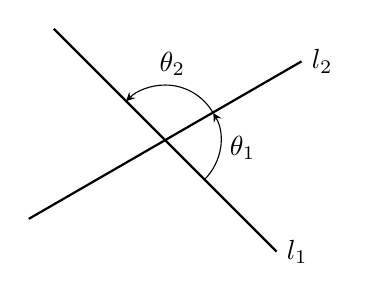
\begin{tikzpicture}[>=stealth, scale=1]
		
		% 1. 绘制直线 \( l_1 \)
		\draw[thick] (0, 0) -- ++(135: 2) ;
		\draw[thick] (0, 0) -- ++(-45: 2) node[ right] {$l_1$};
		% 2. 绘制直线 \( l_2 \)
		\draw[thick] (0, 0) -- ++(30: 2) node[ right] {$l_2$};
		\draw[thick] (0, 0) -- ++(-150: 2) ;
		
		
		% 4. 标记角度 \( \theta_1 \)(\( l_1 \) 与 x 轴正方向的锐角)
		\draw[->] (0.5, -0.5) arc (-45:30:0.7) node[midway, right] {$\theta_1$};
		
		% 5. 标记角度 \( \theta_2 \)(\( l_2 \) 与 x 轴正方向的钝角)
		\draw[->] (0, 0) -- ++(30: 0.7) arc (30:135:0.7) node[midway, above] {$\theta_2$}; 
		
	\end{tikzpicture}
\end{document}
